\documentclass[letter,11pt]{article}
%\documentclass[letter,twoside,11pt]{article}

\usepackage[spanish,es-nodecimaldot]{babel}
\usepackage[utf8]{inputenc}

\usepackage{lmodern}
\usepackage[T1]{fontenc}
\usepackage{textcomp}

\usepackage{framed}
\usepackage[svgnames]{xcolor}
\colorlet{shadecolor}{Gainsboro!50}

\usepackage[labelfont=bf]{caption}
\usepackage{graphicx}
\usepackage{pstricks}

\usepackage{anysize}
\marginsize{3cm}{2cm}{2cm}{3cm}

\usepackage{siunitx}
\usepackage{amsmath}
\usepackage{array}
\usepackage{alltt}

\usepackage{fancyhdr}
\usepackage{lastpage}
\pagestyle{fancy}
\fancyhf{}
\fancyhead[LE,RO]{Laboratorio de Física Básica III}
\fancyfoot[CO,CE]{\thepage\ de \pageref{LastPage}}

\special{papersize=215.9mm,279.4mm}

\usepackage[
    pdfauthor={
        Bastos Lizondo Rosemary;
        Blanco Alconz John Brandon;
        Caballero Burgoa Carlos Eduardo;
        Villena Gutiérrez Ismael Cristian
    },%
    pdftitle={Laboratorio de Física Básica III},%
    pdfsubject={Lineas Equipotenciales},%
    colorlinks,%
    citecolor=black,%
    filecolor=black,%
    linkcolor=black,%
    urlcolor=black,
    breaklinks]{hyperref}
\usepackage{breakurl}

\newcommand{\blankpage}{
\newpage
\thispagestyle{empty}
\mbox{}
\newpage
}

\renewcommand{\arraystretch}{1.2}

\begin{document}

\begin{titlepage}
\begin{center}
{\Large UNIVERSIDAD MAYOR DE SAN SIMÓN}\\
\vspace*{0.15cm}
{\large FACULTAD DE CIENCIAS Y TECNOLOGÍA}\\
\vspace*{0.10cm}
DEPARTAMENTO DE FÍSICA\\
\vspace*{3.0cm}
{\Large \textbf{LABORATORIO DE FÍSICA BÁSICA III}}\\
\vspace*{0.3cm}
{\Large \textbf{INFORME No. 2}}\\
\vspace*{3.5cm}
{\Large \textbf{Lineas Equipotenciales}}\\
\end{center}

\vspace*{6.2cm}
\leftskip=7.95cm
\noindent
\textbf{Integrantes:}\\
Bastos Lizondo Rosemary.\\
Blanco Alconz John Brandon.\\
Caballero Burgoa Carlos Eduardo.\\
Villena Gutiérrez Ismael Cristian.\\
\newline
\textbf{Docente:}\\
Ing. Flores Flores, Freddy.\\
\newline
\textbf{Grupo:} G3.\\
\textbf{Fecha de entrega:} 31 de Marzo del 2021.\\

\end{titlepage}

\section{Evaluación previa}
\begin{enumerate}
\item \textbf{¿Qué relación existe entre el vector campo eléctrico y la línea de
campo eléctrico?} \\
Para cualquier punto, el vector de campo eléctrico es tangente a la línea de
campo eléctrico.

\item \textbf{¿Cómo se define una superficie equipotencial?} \\
Una superficie equipotencial es el lugar geométrico de los puntos de un campo
eléctrico en los cuales el valor del potencial eléctrico es constante. Las
superficies equipotenciales pueden calcularse empleando la ecuación de
\emph{Poisson}.

\item \textbf{¿El campo eléctrico, qué dirección tiene respecto a la superficie
equipotencial?} \\
Para cualquier punto, el campo eléctrico es perpendicular a las superficies
equipotenciales.

\item \textbf{¿Qué es una línea equipotencial?} \\
Las líneas equipotenciales son la representación del potencial eléctrico, dichas
líneas son intersectadas por las líneas de campo formando ángulos rectos. Las
líneas equipotenciales no tienen ninguna dirección definida. Una carga de prueba
situada sobre una línea equipotencial no tiende a seguirla, sino a avanzar hacia
otras de menor potencial. Al contrario que las líneas de campo eléctrico, las
líneas equipotenciales son siempre continuas.

\item \textbf{¿Cuál es la definición de conductividad eléctrica, y cuál es su
unidad de medida?} \\
La conductividad eléctrica ($\sigma$) es la medida de la capacidad de un
material o sustancia para dejar pasar la corriente eléctrica a través de él.
La conductividad es la inversa de la resistividad ($\rho$); por tanto,
$\sigma = 1 / \rho$, y su unidad es el $S/m$ (Siemens por metro) o
$\Omega^{-1} \cdot m^{-1}$.

\item \textbf{¿Qué es un electrodo?} \\
Un electrodo es un conductor eléctrico utilizado para hacer contacto con una
parte no metálica de un circuito, por ejemplo un semiconductor, un electrolito,
el vacío, un gas, etc.

\end{enumerate}

\section{Objetivos}
\begin{itemize}
\item Graficar las líneas equipotenciales para tres configuraciones de carga
(electrodos).
\item Dibujar las líneas de campo eléctrico.
\end{itemize}

\section{Fundamento teórico}

Los vectores de campo eléctrico son tangentes a las líneas de campo eléctrico.
Para una carga puntual positiva las líneas de campo eléctrico están dirigidas
radialmente hacia afuera, y para una carga puntual negativa están dirigidas
radialmente hacia adentro.

Para representar o trazar las líneas de campo se considerará:

\begin{itemize}
\item Las líneas de campo eléctrico no pueden cruzarse entre sí.
\item Deben partir de cargas positivas y terminar en cargas negativas.
\item El número de líneas es proporcional a la magnitud de la carga que la
produce.
\item La separación entre las líneas de campo determina la intensidad de campo
eléctrico.
\end{itemize}

Una superficie equipotencial (o líneas equipotenciales en el caso de una
dimensión), es aquella superficie (o línea) en la que todos sus puntos tienen el
mismo potencial eléctrico. Las superficies equipotenciales de una carga puntual
son esferas concéntricas, y para un capacitor de placas paralelas son planos
paralelos a las placas.

El campo eléctrico intercepta perpendicularmente a las superficies
equipotenciales, esto puede demostrarse a partir de la definición de superficie
equipotencial y del gradiente del potencial eléctrico:

\begin{equation}
    E = - \nabla V
\end{equation}
\begin{equation}
    E \cdot dr = - \nabla V \cdot dr = - dV
\end{equation}

\section{Materiales}
\begin{itemize}
\item Simulador «PhET Interactive Simulations» Cargas y campos.
\end{itemize}

\section{Procedimiento experimental}
Se establecieron tres configuraciones para los electrodos:

\begin{enumerate}
\item Dos cargas puntuales de signos opuestos.
\item Una carga puntual y una línea de cargas.
\item Dos líneas de carga de signos opuestos.
\end{enumerate}

Y para cada configuración se realizaron los siguientes pasos:

\begin{enumerate}
\item Ir al simulador ubicado en la dirección web:
(https://phet.colorado.edu/sims/html/charges-and-fields/latest/charges-and-fields\_es.html),
tal como se muestra en la \textbf{Figura \ref{figura1}}.

\begin{figure}[!h]
\centering

\includegraphics[scale=0.34]{resources/figura01.eps}
\caption{Simulador para cargas y campos eléctricos.}
\label{figura1}
\end{figure}
\item Fijar una distancia de separación entre cargas.
\item Formar la configuración, con las cargas puntuales necesarias.
\item Habilitar el «voltaje» en el simulador.
\item Elegir un voltaje a encontrar entre los electrodos, y escoger puntos
($x$, $y$) correspondientes a potenciales semejantes al valor elegido.
\item Completar las tablas correspondientes para cada configuración, con los
diferentes potenciales escogidos.
\item Graficar las líneas equipotenciales según los datos recolectados.
\item Graficar las lineas de campo eléctrico.
\end{enumerate}

\section{Resultados}

\textbf{\underline{Configuración 1}}: Dos cargas puntuales de signos opuestos. \\

En la \textbf{Figura \ref{figura2}} se muestra la disposición de las cargas y el
sistema de referencia utilizado.

\begin{figure}[!h]
\centering
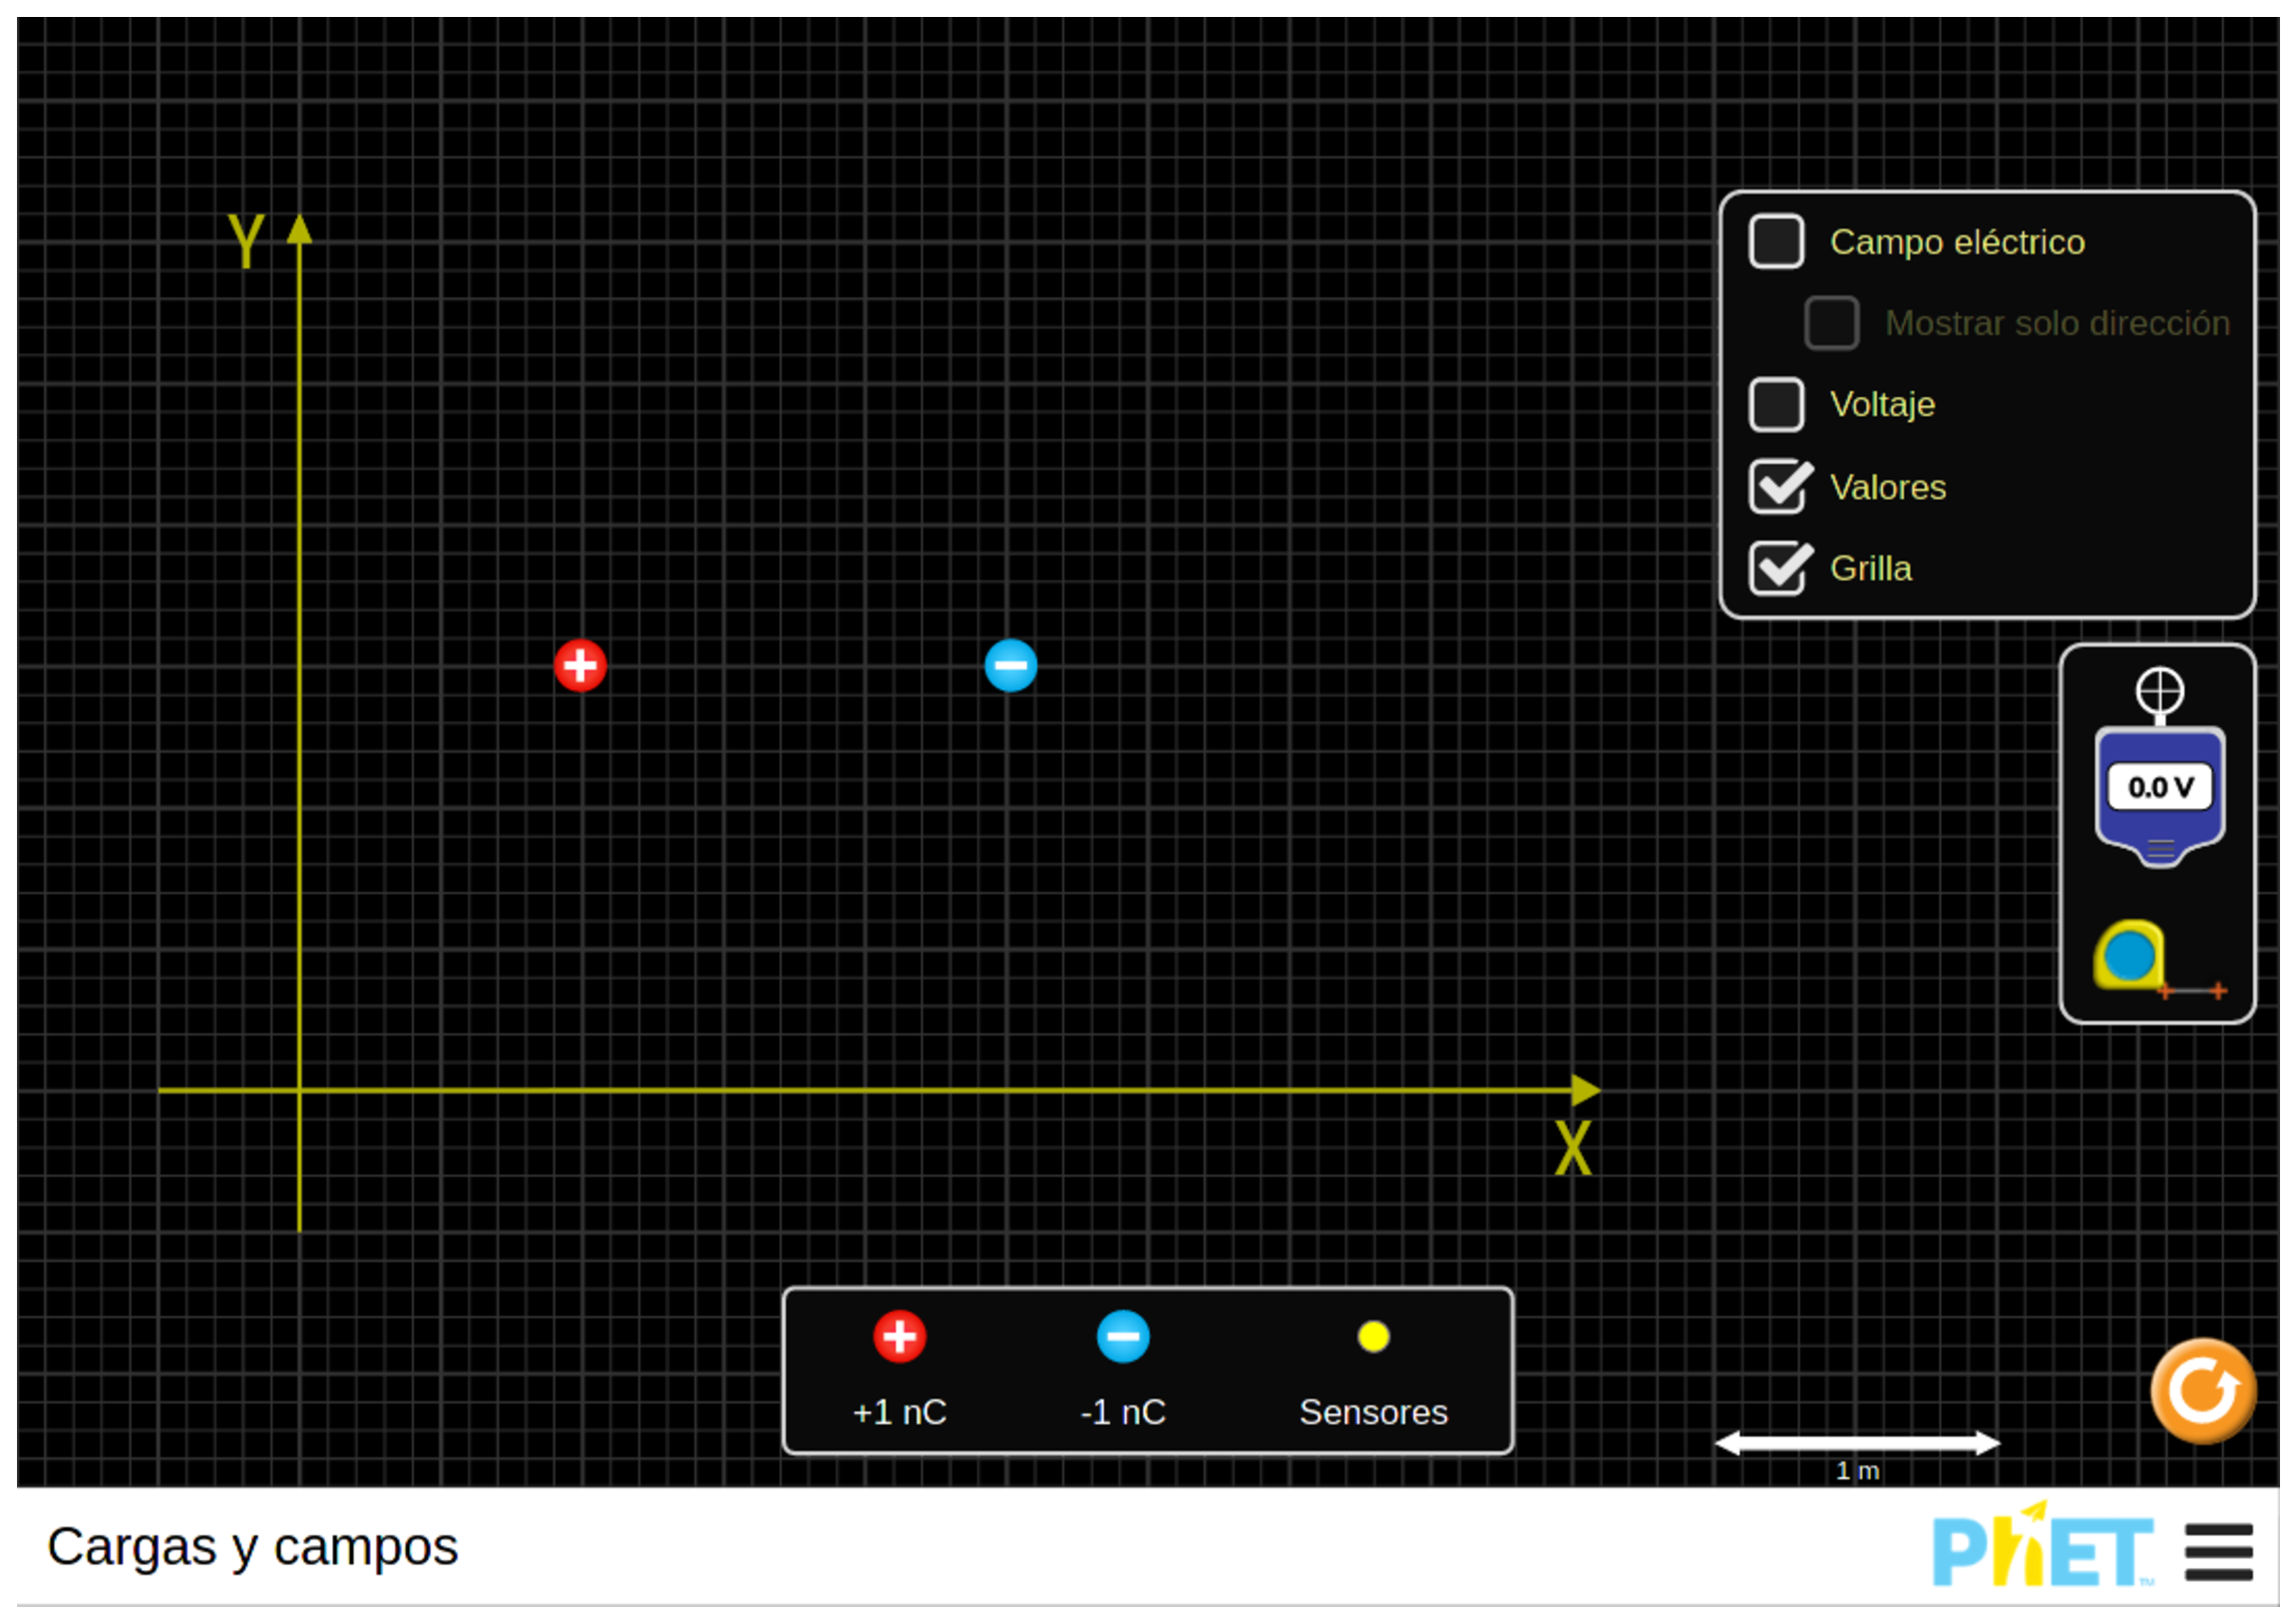
\includegraphics[scale=0.34]{resources/figura02.eps}
\caption{Dos cargas puntuales de signos opuestos.}
\label{figura2}
\end{figure}

Distancia de separación entre las cargas:

\begin{equation*}
    d = 150 [cm]
\end{equation*}

Valor y posición de la carga 1:

\begin{equation*}
    Q_1 = +7 [nC]
\end{equation*}
\begin{equation*}
    X_1 = 100 [cm]
\end{equation*}
\begin{equation*}
    Y_1 = 150 [cm]
\end{equation*}

Valor y posición de la carga 2:

\begin{equation*}
    Q_2 = -7 [nC]
\end{equation*}
\begin{equation*}
    X_2 = 250 [cm]
\end{equation*}
\begin{equation*}
    Y_2 = 150 [cm]
\end{equation*}

Los valores de potencial eléctrico recogidos en el simulador pueden verse
gráficamente en la \textbf{Figura \ref{figura3}}.

\begin{figure}[!h]
\centering

\includegraphics[scale=0.34]{resources/figura03.eps}
\caption{Lineas equipotenciales elegidas para la configuración 1.}
\label{figura3}
\end{figure}

En el \textbf{Cuadro \ref{cuadro1}}, se muestran los valores de las coordenadas
($x$, $y$) para los voltajes elegidos.

\begin{table}[!h]
\begin{center}
\begin{tabular}{|c||>{\centering}m{1.7cm}<{\centering}
                   |>{\centering}m{1.7cm}<{\centering}|
                   |>{\centering}m{1.7cm}<{\centering}
                   |>{\centering}m{1.7cm}<{\centering}|
                   |>{\centering}m{1.7cm}<{\centering}
                   |>{\centering}m{1.7cm}<{\centering}|}
\hline
    & \multicolumn{2}{c||}{$V_1 = 11.7 [V] $} & \multicolumn{2}{c||}{$V_2 = 23.3 [V] $} & \multicolumn{2}{c|}{$V_3 = 102.7 [V] $} \\
\hline
$i$ & $x_i [cm]$ & $y_i [cm]$ & $x_i [cm]$ & $y_i [cm]$ & $x_i [cm]$ & $y_i [cm]$ \tabularnewline \hline
1 & -50 & 292.1 &  10 & 248.1 &  70 & 185.2 \tabularnewline \hline
2 &  50 & 319.2 &  90 & 262.8 & 100 & 194.6 \tabularnewline \hline
3 & 150 & 249.2 & 150 & 214.5 & 120 & 186.9 \tabularnewline \hline
4 & 150 &  51.2 & 150 &  82.9 & 120 & 113.5 \tabularnewline \hline
5 &  50 & -19.4 &  90 &  37.0 & 100 & 105.8 \tabularnewline \hline
6 & -50 &   9.4 &  10 &  52.3 &  70 & 114.0 \tabularnewline \hline
\hline
& \multicolumn{2}{c||}{$V_4 = -11.3 [V] $} & \multicolumn{2}{c||}{$V_5 = -23.4 [V] $} & \multicolumn{2}{c|}{$V_6 = -97.8 [V] $} \\
\hline
$i$ & $x_i [cm]$ & $y_i [cm]$ & $x_i [cm]$ & $y_i [cm]$ & $x_i [cm]$ & $y_i [cm]$ \tabularnewline \hline
1 & 200 & 252.8 & 200 & 215.7 & 230 & 189.9 \tabularnewline \hline
2 & 300 & 322.7 & 270 & 265.7 & 250 & 195.2 \tabularnewline \hline
3 & 400 &   3.5 & 340 & 247.5 & 280 & 187.5 \tabularnewline \hline
4 & 400 & 297.4 & 340 &  52.9 & 280 & 114.0 \tabularnewline \hline
5 & 300 & -23.0 & 270 &  35.3 & 250 & 104.0 \tabularnewline \hline
6 & 200 &  47.6 & 200 &  84.1 & 230 & 112.3 \tabularnewline \hline
\end{tabular}
\caption{Coordenadas de las mediciones para diferentes voltajes.}
\label{cuadro1}
\end{center}
\end{table}

Sabiendo que las líneas de campo eléctrico son perpendiculares a las líneas
equipotenciales, obtenemos la gráfica de la \textbf{Figura \ref{figura4}}.

\begin{figure}[!h]
\centering
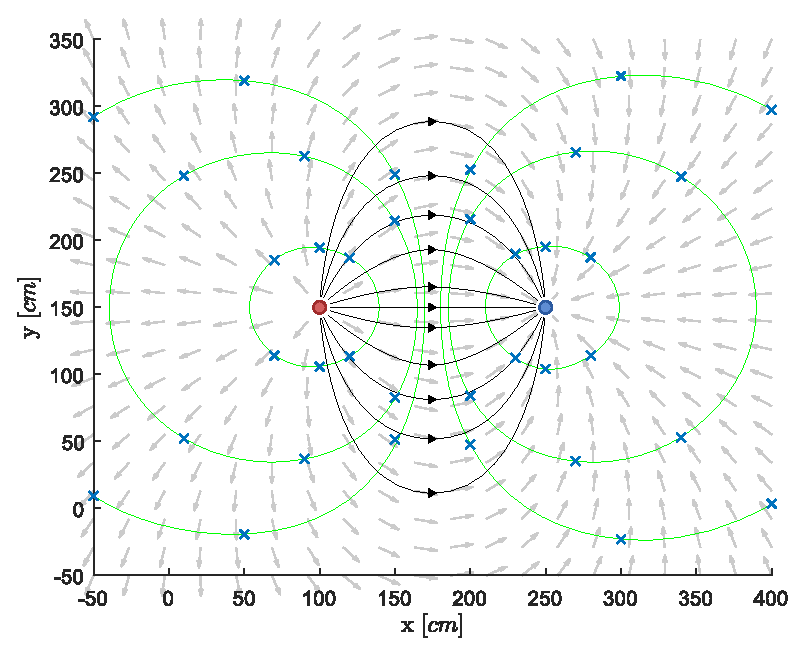
\includegraphics[scale=0.91]{resources/p1.eps}
\caption{Lineas de campo eléctrico para la configuración 1.}
\label{figura4}
\end{figure}

\vspace{0.45cm}
\textbf{\underline{Configuración 2}}: Una carga puntual y una linea de cargas. \\

En la \textbf{Figura \ref{figura5}} se muestra la disposición de las cargas y el
sistema de referencia utilizado.

\begin{figure}[!h]
\centering
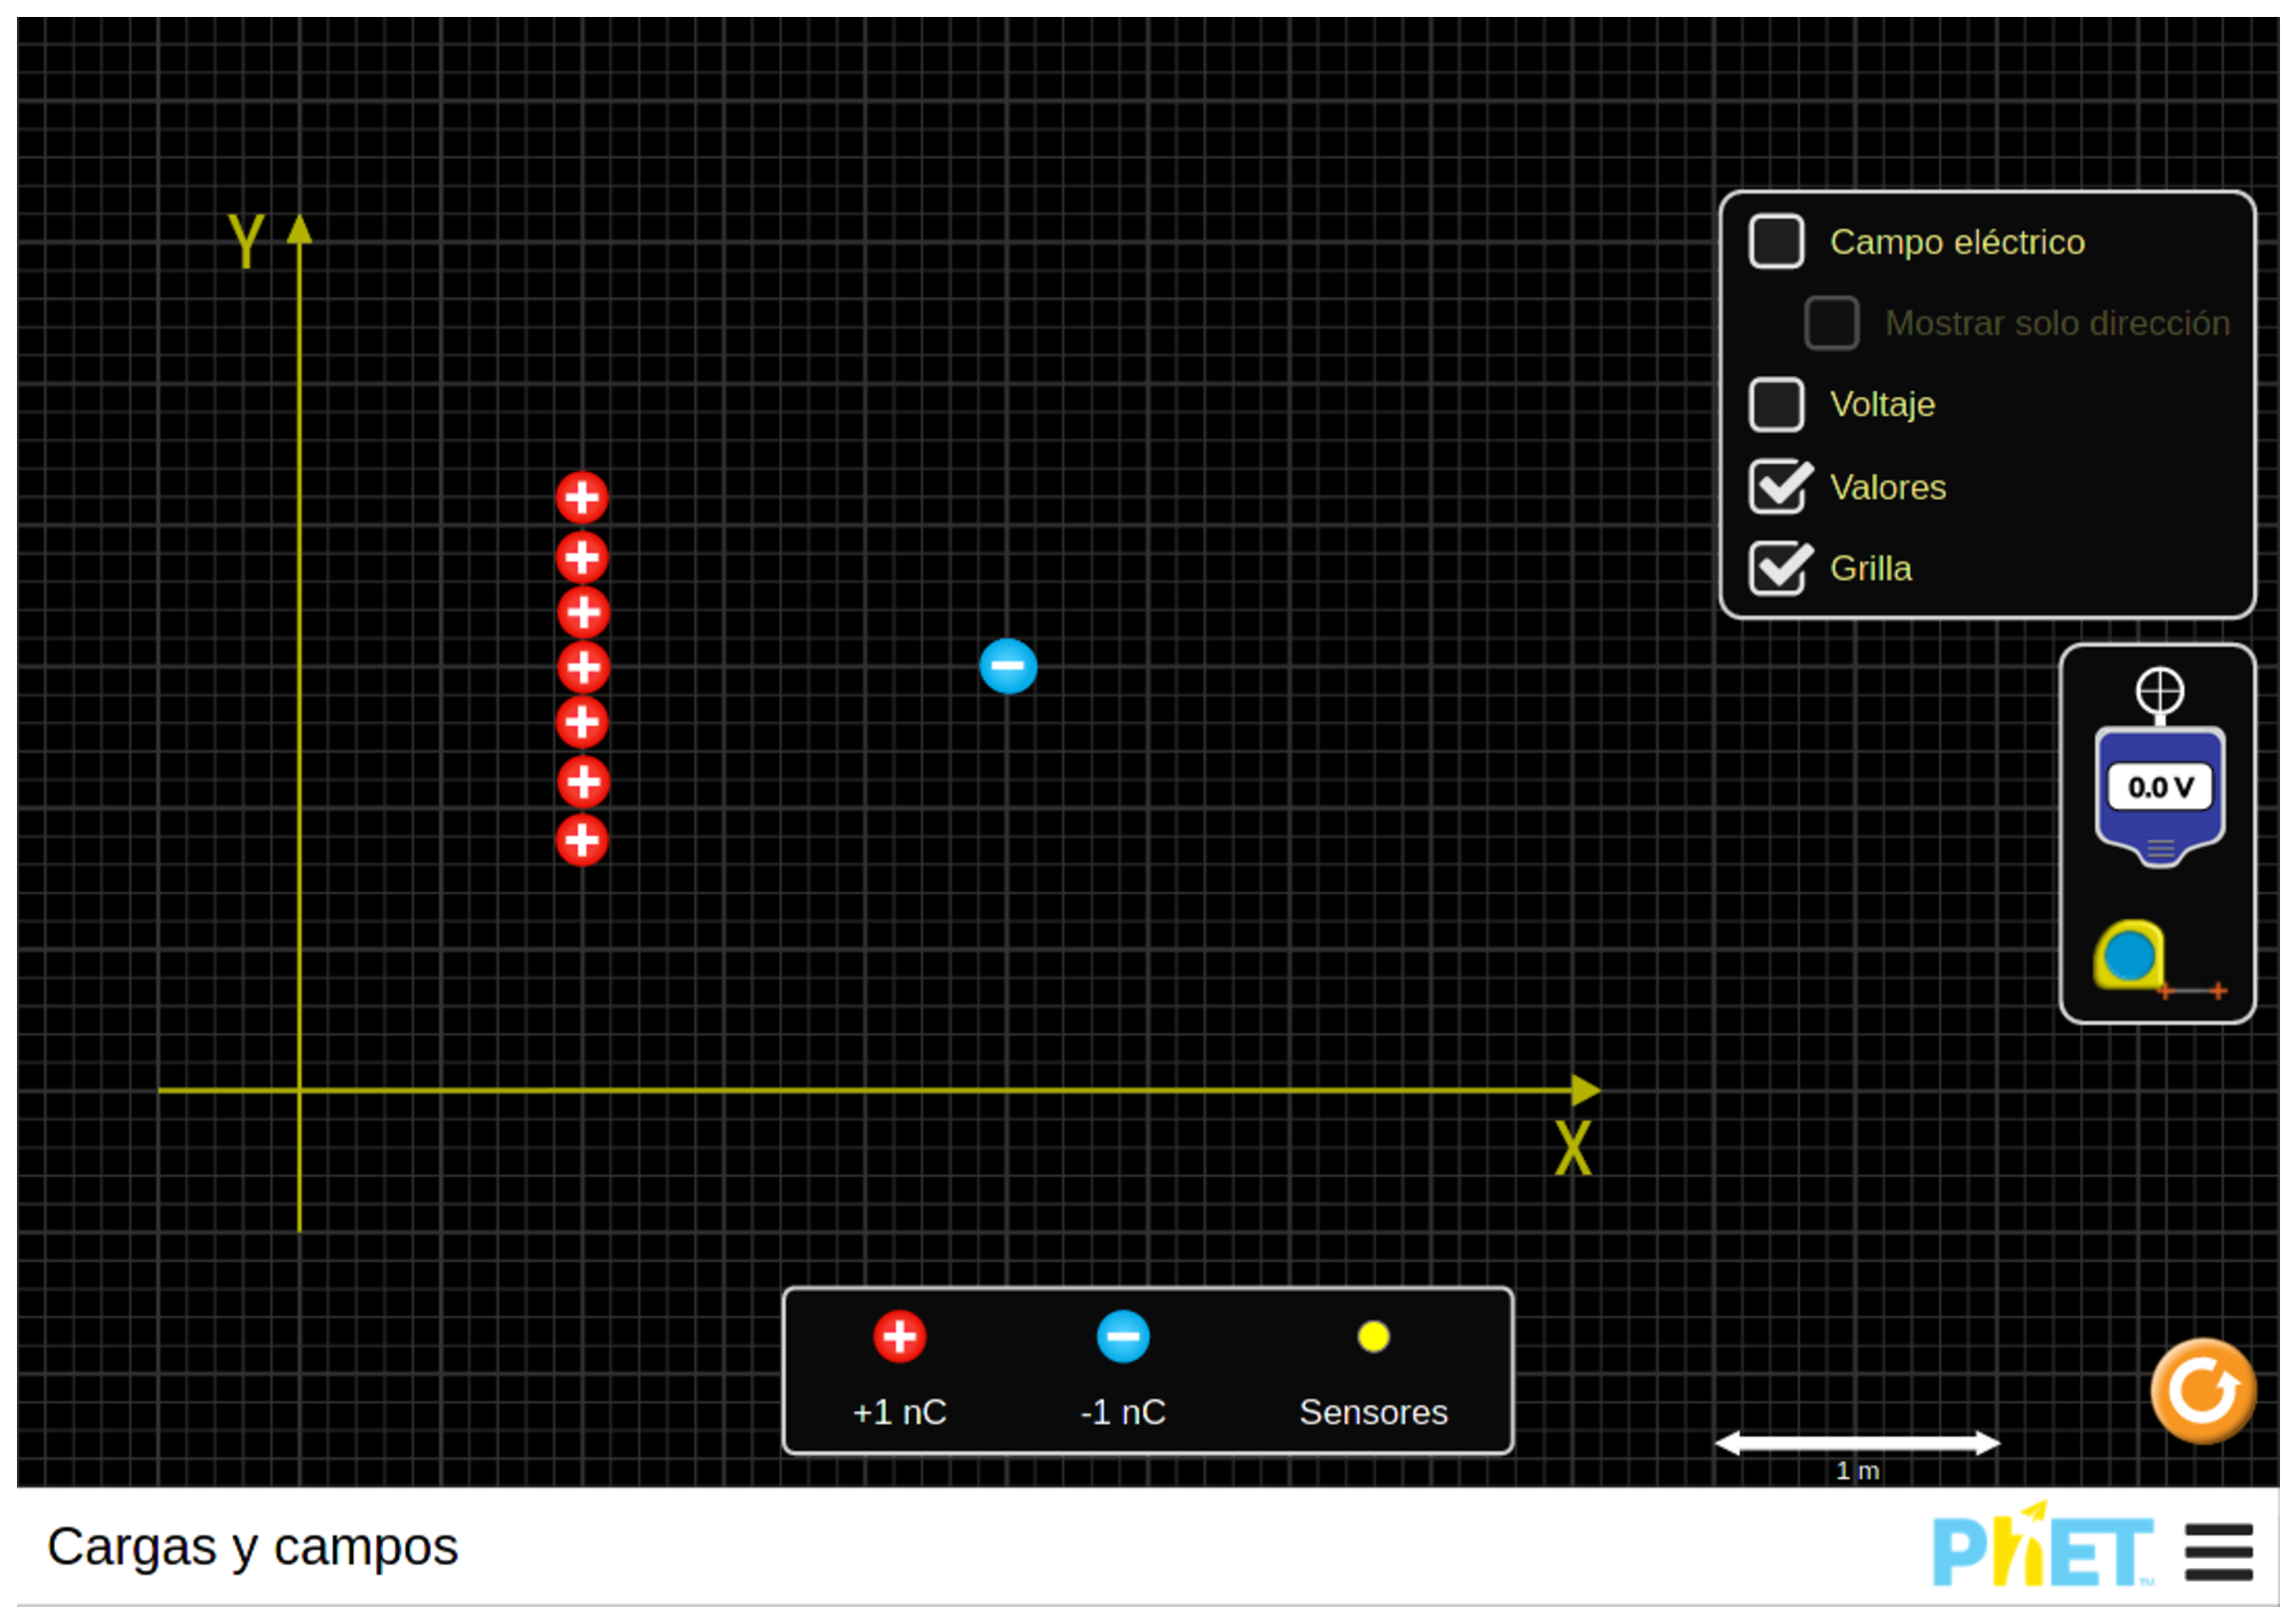
\includegraphics[scale=0.34]{resources/figura05.eps}
\caption{Configuración de una carga puntual y una linea de cargas.}
\label{figura5}
\end{figure}

Distancia de separación horizontal entre las cargas:

\begin{equation*}
    d = 150 [cm]
\end{equation*}

Valor y posiciones de la linea de carga 1:

\begin{equation*}
    Q_1 = +1 [nC]
\end{equation*}
\begin{equation*}
    X_{1.1} = 100 [cm]; Y_{1.1} = 90 [cm]
\end{equation*}
\begin{equation*}
    X_{1.2} = 100 [cm]; Y_{1.2} = 110 [cm]
\end{equation*}
\begin{equation*}
    X_{1.3} = 100 [cm]; Y_{1.3} = 130 [cm]
\end{equation*}
\begin{equation*}
    X_{1.4} = 100 [cm]; Y_{1.4} = 150 [cm]
\end{equation*}
\begin{equation*}
    X_{1.5} = 100 [cm]; Y_{1.5} = 170 [cm]
\end{equation*}
\begin{equation*}
    X_{1.6} = 100 [cm]; Y_{1.6} = 190 [cm]
\end{equation*}
\begin{equation*}
    X_{1.7} = 100 [cm]; Y_{1.7} = 210 [cm]
\end{equation*}

Valor y posición de la carga 2:

\begin{equation*}
    Q_2 = -7 [nC]
\end{equation*}
\begin{equation*}
    X_2 = 250 [cm]
\end{equation*}
\begin{equation*}
    Y_2 = 150 [cm]
\end{equation*}

Los valores de potencial eléctrico recogidos en el simulador pueden verse
gráficamente en la \textbf{Figura \ref{figura6}}.

\begin{figure}[!h]
\centering
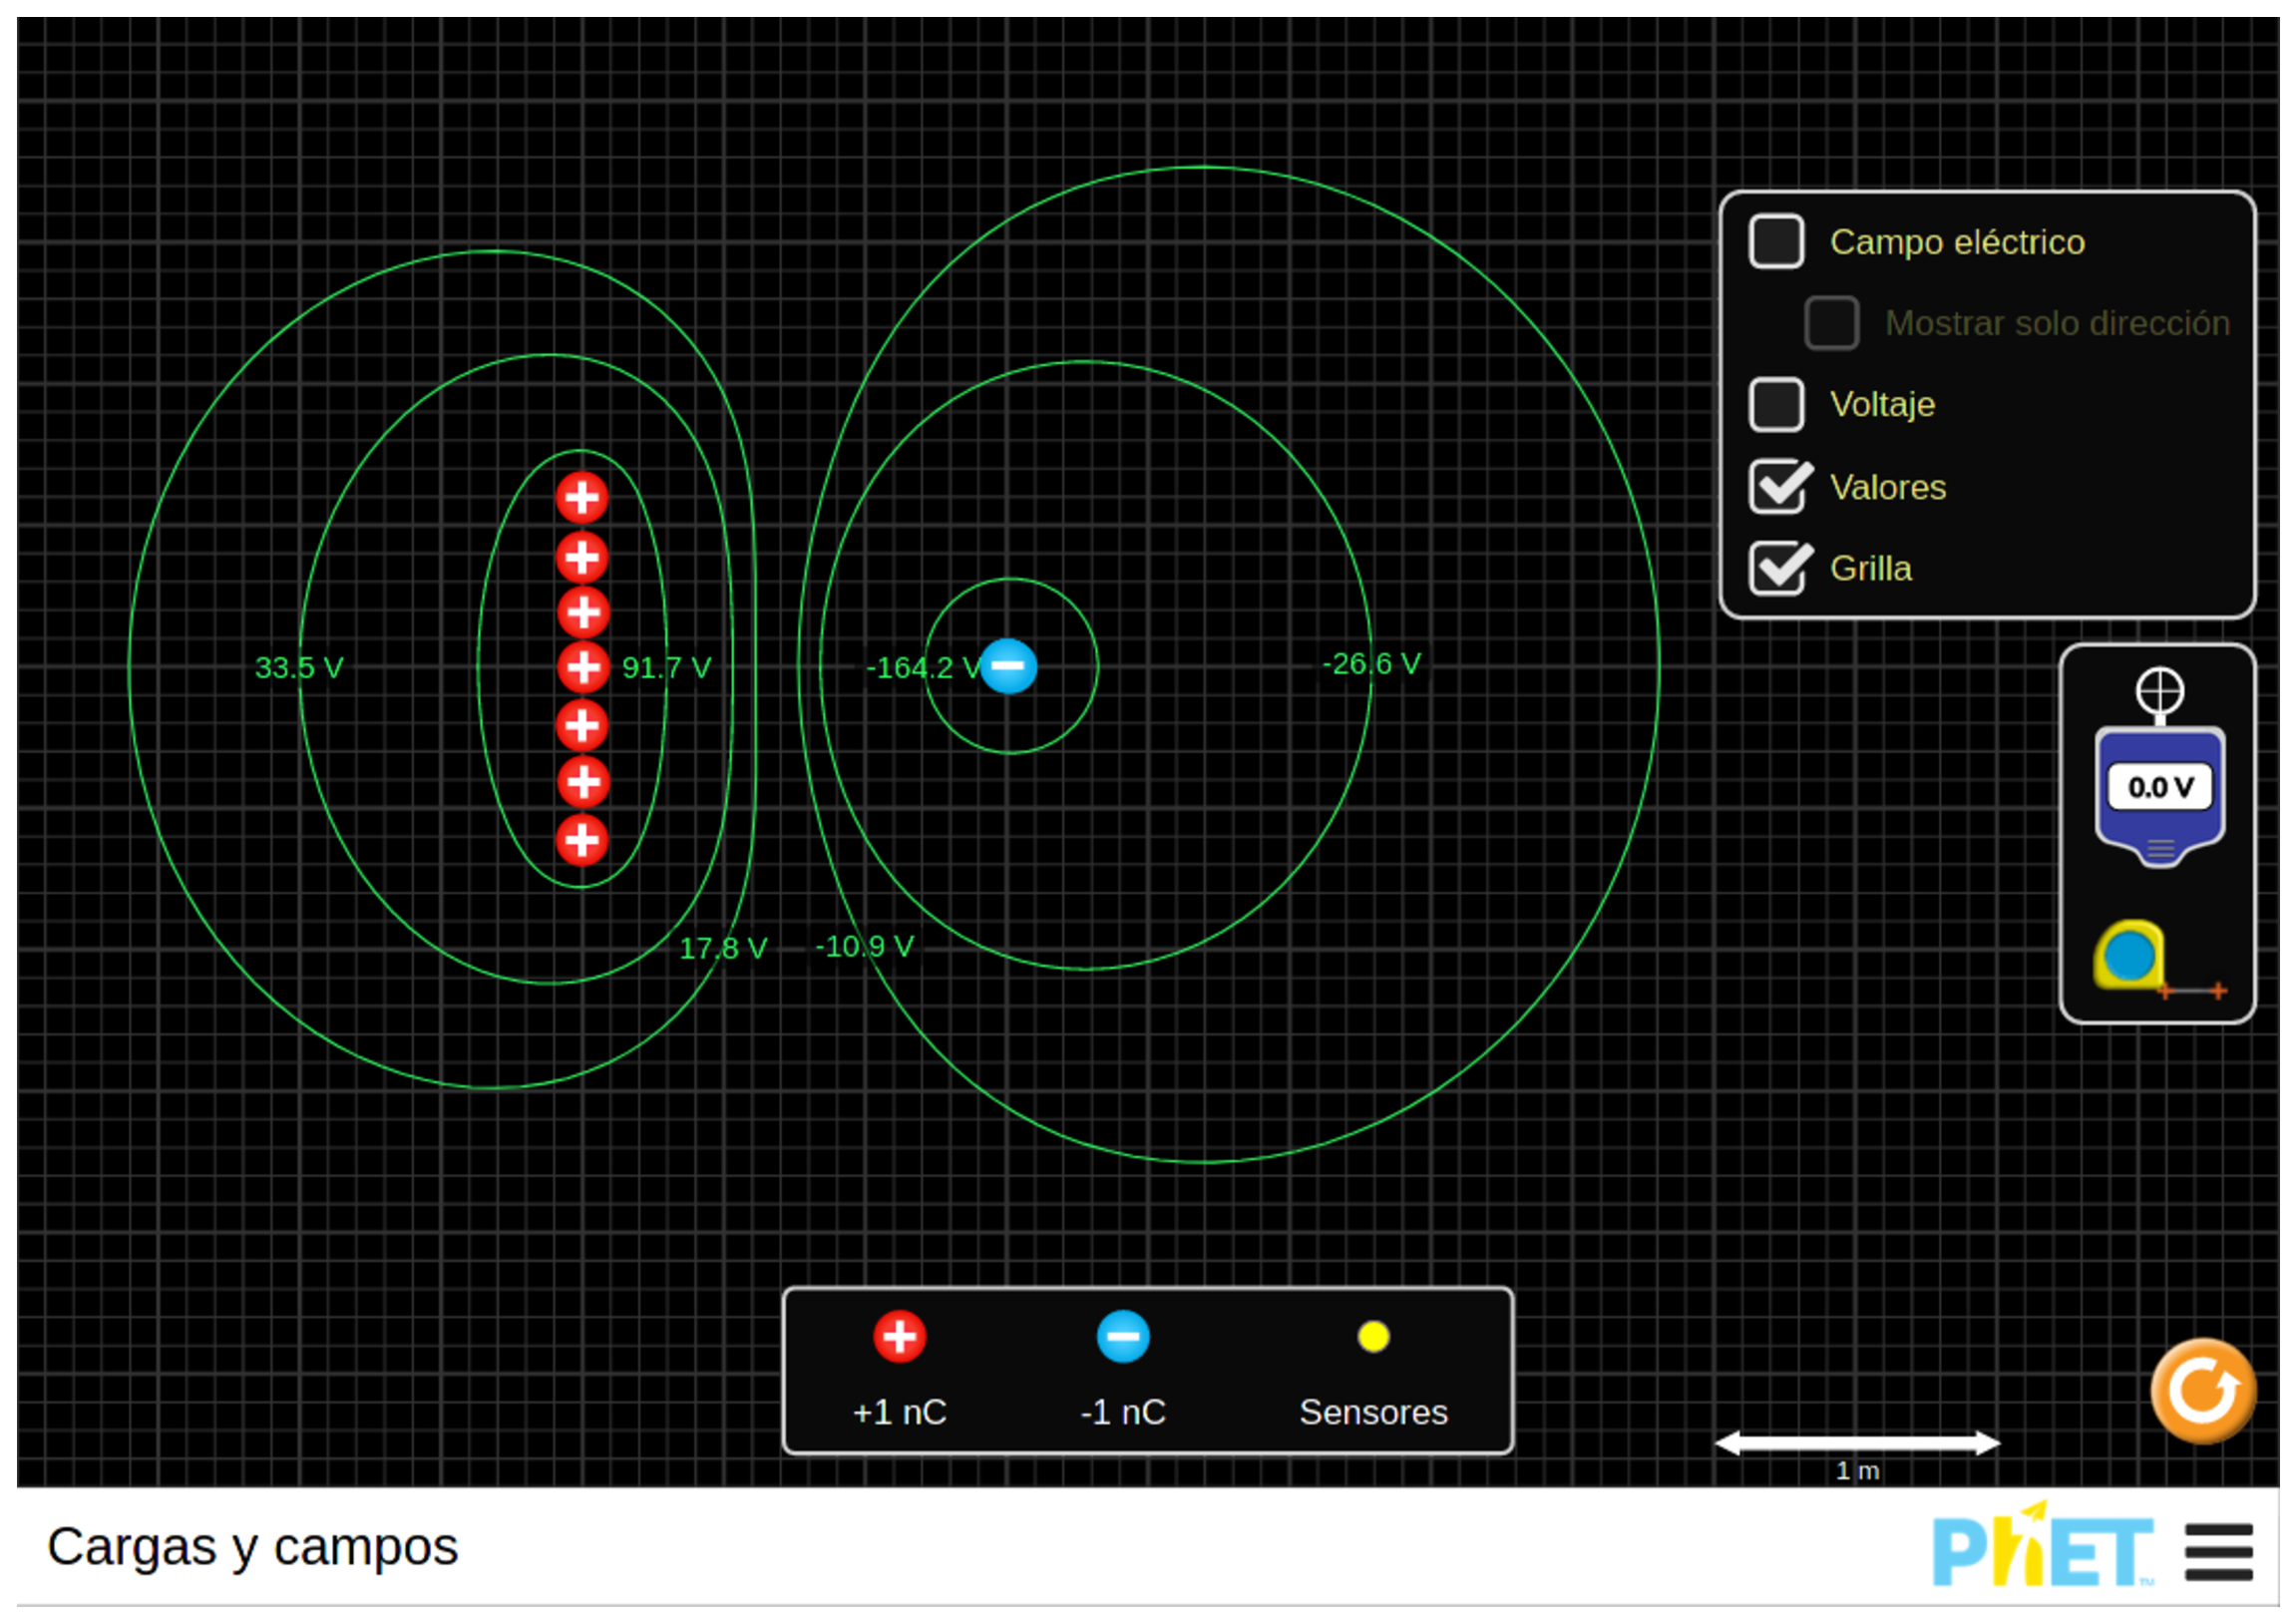
\includegraphics[scale=0.34]{resources/figura06.eps}
\caption{Lineas equipotenciales para la configuración 2.}
\label{figura6}
\end{figure}

En el \textbf{Cuadro \ref{cuadro2}}, se muestran los valores de las coordenadas
($x$, $y$) para los voltajes elegidos.

\begin{table}[!h]
\begin{center}
\begin{tabular}{|c||>{\centering}m{1.7cm}<{\centering}
                   |>{\centering}m{1.7cm}<{\centering}|
                   |>{\centering}m{1.7cm}<{\centering}
                   |>{\centering}m{1.7cm}<{\centering}|
                   |>{\centering}m{1.7cm}<{\centering}
                   |>{\centering}m{1.7cm}<{\centering}|}
\hline
& \multicolumn{2}{c||}{$V_1 = 17.8 [V] $} & \multicolumn{2}{c||}{$V_2 = 33.5 [V] $} & \multicolumn{2}{c|}{$V_3 = 91.7 [V] $} \\
\hline
$i$ & $x_i [cm]$ & $y_i [cm]$ & $x_i [cm]$ & $y_i [cm]$ & $x_i [cm]$ & $y_i [cm]$ \tabularnewline \hline
1 & -50 & 205.7 &  10 & 197.4 &  70 & 194.0 \tabularnewline \hline
2 &  50 &   3.4 &  90 & 259.2 & 100 & 227.5 \tabularnewline \hline
3 & 150 & 247.4 & 150 & 194.5 & 120 & 209.8 \tabularnewline \hline
4 & 150 &  52.3 & 150 & 102.8 & 120 &  88.1 \tabularnewline \hline
5 &  50 & 295.6 &  90 &  37.0 & 100 &  72.3 \tabularnewline \hline
6 & -50 &  91.6 &  10 &  99.3 &  70 & 104.6 \tabularnewline \hline
\hline
& \multicolumn{2}{c||}{$V_4 = -10.9 [V] $} & \multicolumn{2}{c||}{$V_5 = -26.6 [V] $} & \multicolumn{2}{c|}{$V_6 = -164.2 [V] $} \\
\hline
$i$ & $x_i [cm]$ & $y_i [cm]$ & $x_i [cm]$ & $y_i [cm]$ & $x_i [cm]$ & $y_i [cm]$ \tabularnewline \hline
1 & 200 & 252.1 & 200 & 211.5 & 230 & 171.6 \tabularnewline \hline
2 & 300 & 325.0 & 270 & 257.4 & 250 & 181.6 \tabularnewline \hline
3 & 400 & 302.7 & 340 & 234.5 & 280 & 158.6 \tabularnewline \hline
4 & 400 &   0   & 340 &  66.4 & 280 & 139.8 \tabularnewline \hline
5 & 300 & -25.3 & 270 &  44.0 & 250 & 119.3 \tabularnewline \hline
6 & 200 &  49.3 & 200 &  88.1 & 230 & 127.5 \tabularnewline \hline
\end{tabular}
\caption{Coordenadas de las mediciones para diferentes voltajes.}
\label{cuadro2}
\end{center}
\end{table}

Sabiendo que las líneas de campo eléctrico son perpendiculares a las líneas
equipotenciales, obtenemos la gráfica de la \textbf{Figura \ref{figura7}}.

\begin{figure}[!h]
\centering
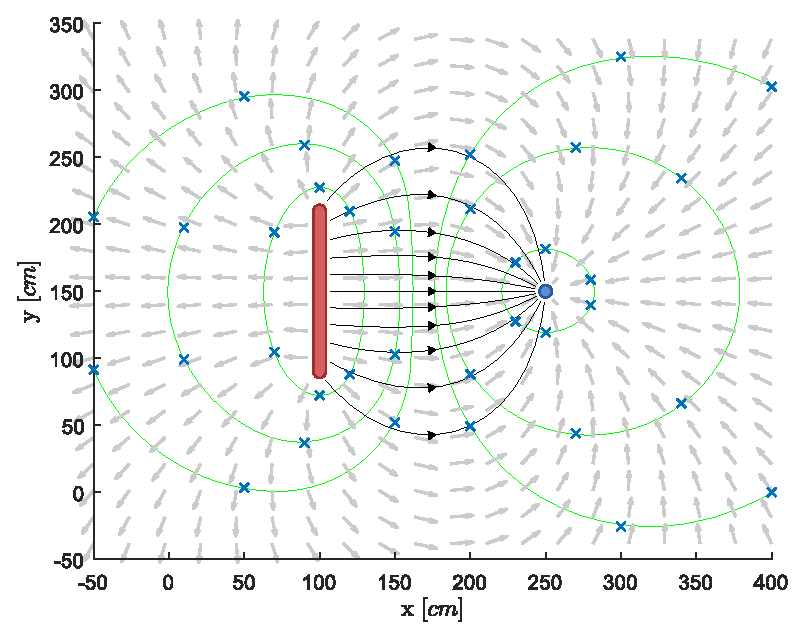
\includegraphics[scale=0.91]{resources/p2.eps}
\caption{Lineas de campo eléctrico para la configuración 2.}
\label{figura7}
\end{figure}

\vspace{0.45cm}
\textbf{\underline{Configuración 3}}: Dos cargas puntuales de signos opuestos. \\

En la \textbf{Figura \ref{figura8}} se muestra la disposición de las cargas y el
sistema de referencia utilizado.

\begin{figure}[!h]
\centering
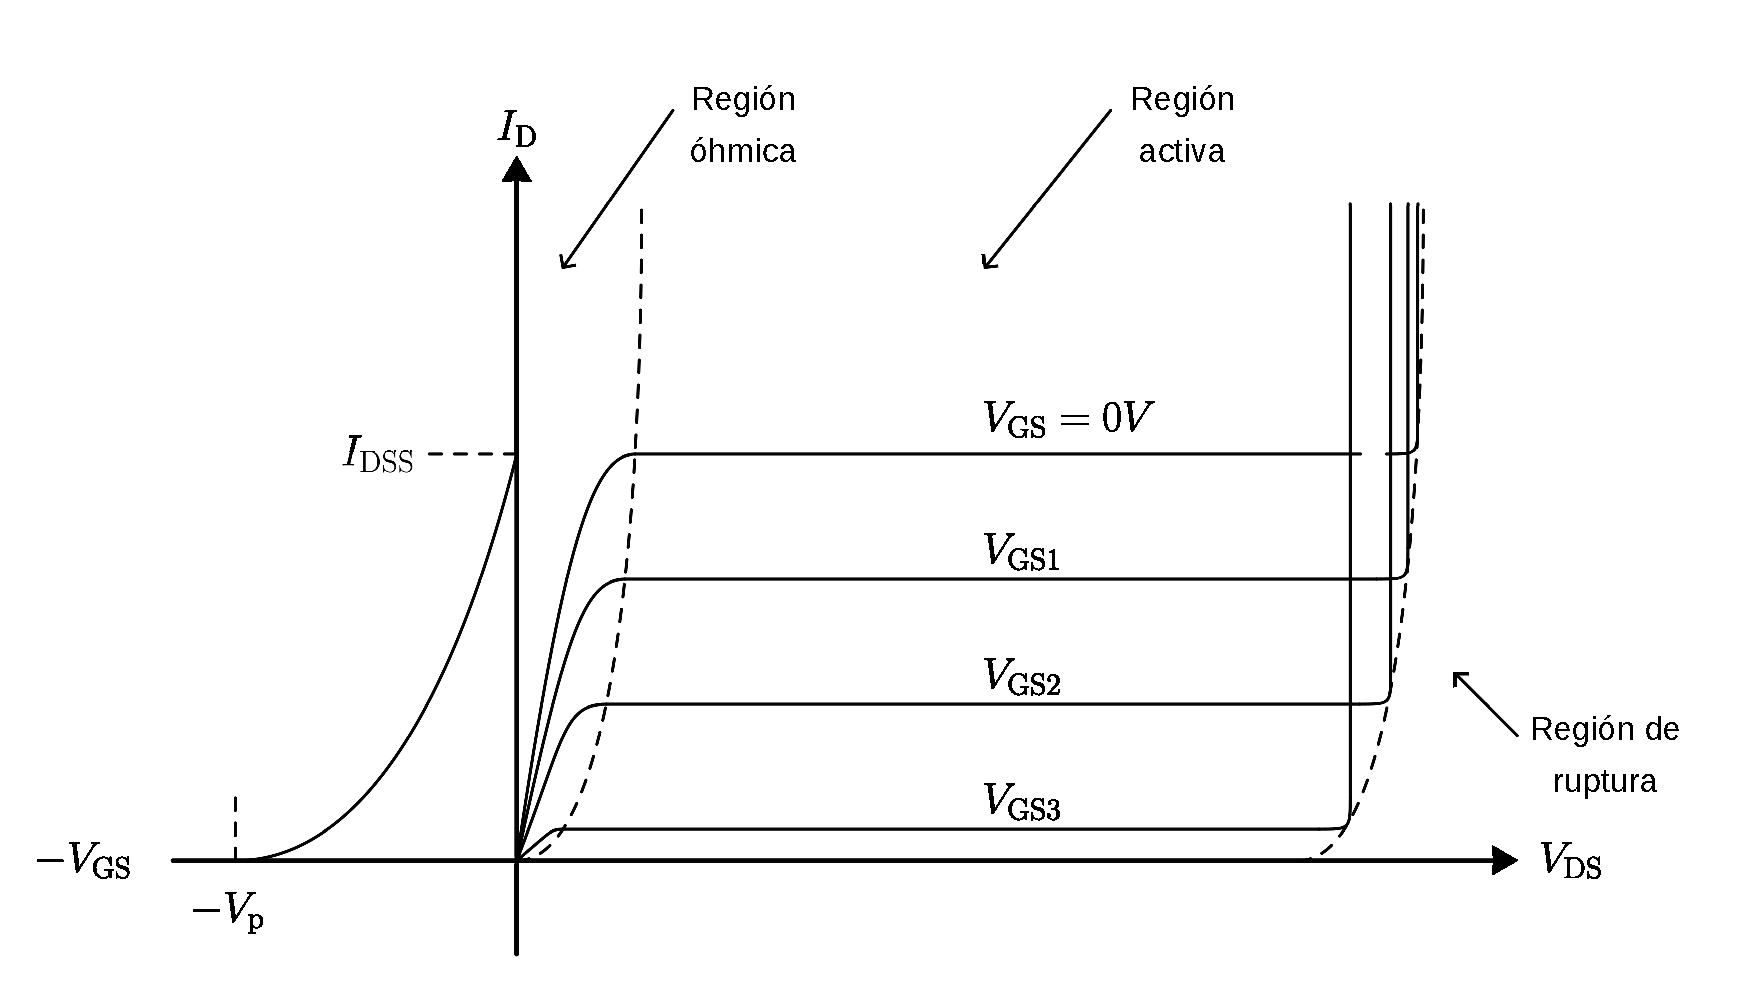
\includegraphics[scale=0.34]{resources/figura08.eps}
\caption{Configuración de dos lineas de carga de signos opuestos.}
\label{figura8}
\end{figure}

Distancia de separación horizontal entre las cargas:

\begin{equation*}
    d = 150 [cm]
\end{equation*}

Valor y posiciones de la linea de carga 1:

\begin{equation*}
    Q_1 = +1 [nC]
\end{equation*}
\begin{equation*}
    X_{1.1} = 100 [cm]; Y_{1.1} = 90 [cm]
\end{equation*}
\begin{equation*}
    X_{1.2} = 100 [cm]; Y_{1.2} = 110 [cm]
\end{equation*}
\begin{equation*}
    X_{1.3} = 100 [cm]; Y_{1.3} = 130 [cm]
\end{equation*}
\begin{equation*}
    X_{1.4} = 100 [cm]; Y_{1.4} = 150 [cm]
\end{equation*}
\begin{equation*}
    X_{1.5} = 100 [cm]; Y_{1.5} = 170 [cm]
\end{equation*}
\begin{equation*}
    X_{1.6} = 100 [cm]; Y_{1.6} = 190 [cm]
\end{equation*}
\begin{equation*}
    X_{1.7} = 100 [cm]; Y_{1.7} = 210 [cm]
\end{equation*}

Valor y posiciones de la linea de carga 2:

\begin{equation*}
    Q_1 = -1 [nC]
\end{equation*}
\begin{equation*}
    X_{2.1} = 250 [cm]; Y_{2.1} = 90 [cm]
\end{equation*}
\begin{equation*}
    X_{2.2} = 250 [cm]; Y_{2.2} = 110 [cm]
\end{equation*}
\begin{equation*}
    X_{2.3} = 250 [cm]; Y_{2.3} = 130 [cm]
\end{equation*}
\begin{equation*}
    X_{2.4} = 250 [cm]; Y_{2.4} = 150 [cm]
\end{equation*}
\begin{equation*}
    X_{2.5} = 250 [cm]; Y_{2.5} = 170 [cm]
\end{equation*}
\begin{equation*}
    X_{2.6} = 250 [cm]; Y_{2.6} = 190 [cm]
\end{equation*}
\begin{equation*}
    X_{2.7} = 250 [cm]; Y_{2.7} = 210 [cm]
\end{equation*}

Los valores potencial eléctrico recogidos en el simulador pueden verse
gráficamente en la \textbf{Figura \ref{figura9}}.

\begin{figure}[!h]
\centering
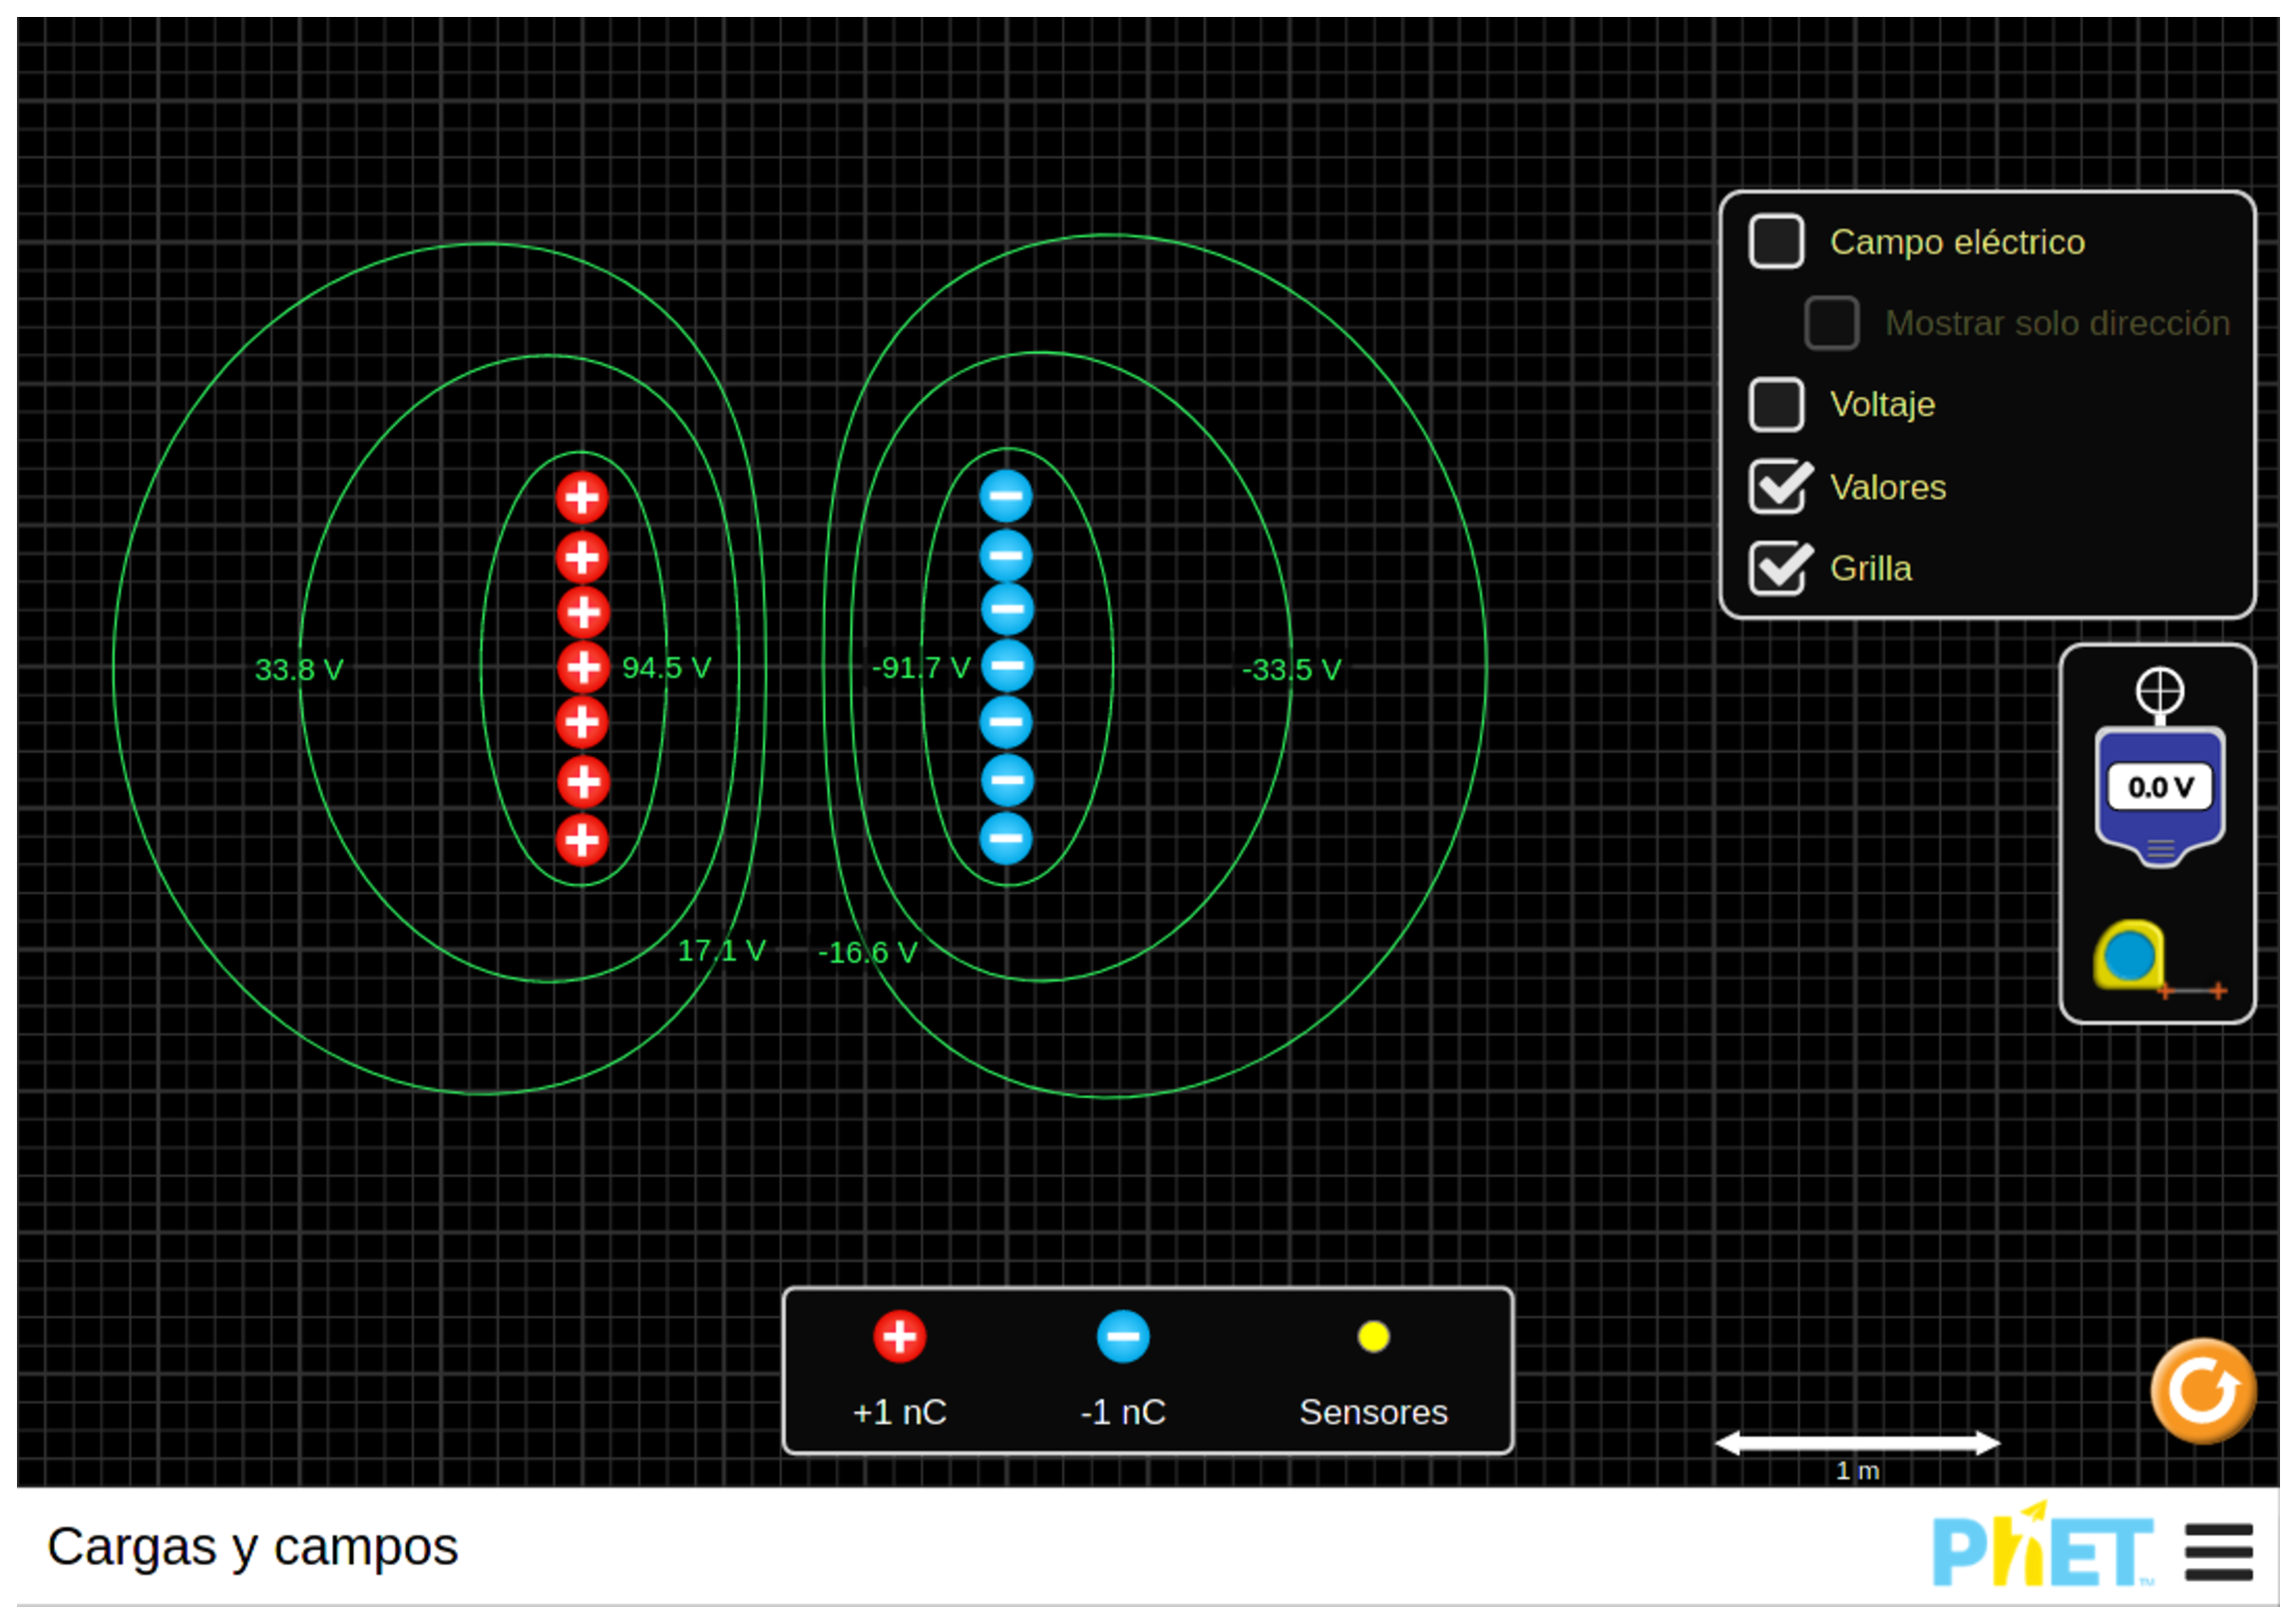
\includegraphics[scale=0.34]{resources/figura09.eps}
\caption{Lineas equipotenciales para la configuración 3.}
\label{figura9}
\end{figure}

En el \textbf{Cuadro \ref{cuadro3}}, se muestran los valores de las coordenadas
($x$, $y$) para los voltajes elegidos.

\begin{table}[!h]
\begin{center}
\begin{tabular}{|c||>{\centering}m{1.7cm}<{\centering}
                   |>{\centering}m{1.7cm}<{\centering}|
                   |>{\centering}m{1.7cm}<{\centering}
                   |>{\centering}m{1.7cm}<{\centering}|
                   |>{\centering}m{1.7cm}<{\centering}
                   |>{\centering}m{1.7cm}<{\centering}|}
\hline
& \multicolumn{2}{c||}{$V_1 = 17.1 [V] $} & \multicolumn{2}{c||}{$V_2 = 33.8 [V] $} & \multicolumn{2}{c|}{$V_3 = 94.5 [V] $} \\
\hline
$i$ & $x_i [cm]$ & $y_i [cm]$ & $x_i [cm]$ & $y_i [cm]$ & $x_i [cm]$ & $y_i [cm]$ \tabularnewline \hline
1 & -50 & 221.0 &  10 & 198.7 &  70 & 192.8 \tabularnewline \hline
2 &  50 & 298.6 &  90 & 260.4 & 100 & 225.7 \tabularnewline \hline
3 & 150 & 243.9 & 150 & 202.2 & 120 & 207.5 \tabularnewline \hline
4 & 150 &  51.7 & 150 &  95.2 & 120 &  88.8 \tabularnewline \hline
5 &  50 &   0   &  90 &  38.8 & 100 &  72.3 \tabularnewline \hline
6 & -50 &  79.9 &  10 &  99.9 &  70 & 108.2 \tabularnewline \hline
\hline
& \multicolumn{2}{c||}{$V_4 = -16.6 [V] $} & \multicolumn{2}{c||}{$V_5 = -33.5 [V] $} & \multicolumn{2}{c|}{$V_6 = -91.7 [V] $} \\
\hline
$i$ & $x_i [cm]$ & $y_i [cm]$ & $x_i [cm]$ & $y_i [cm]$ & $x_i [cm]$ & $y_i [cm]$ \tabularnewline \hline
1 & 200 & 249.8 & 200 & 205.1 & 230 & 213.4 \tabularnewline \hline
2 & 300 & 301.5 & 270 & 261.0 & 250 & 227.5 \tabularnewline \hline
3 & 400 & 226.3 & 340 & 203.4 & 280 & 195.2 \tabularnewline \hline
4 & 400 &  71.7 & 340 &  96.4 & 280 & 104.0 \tabularnewline \hline
5 & 300 &   0   & 270 &  39.4 & 250 &  73.5 \tabularnewline \hline
6 & 200 &  51.7 & 200 &  96.4 & 230 &  88.8 \tabularnewline \hline
\end{tabular}
\caption{Coordenadas de las mediciones para diferentes voltajes.}
\label{cuadro3}
\end{center}
\end{table}

Sabiendo que las líneas de campo eléctrico son perpendiculares a las líneas
equipotenciales, obtenemos la gráfica de la \textbf{Figura \ref{figura10}}.

\begin{figure}[!h]
\centering
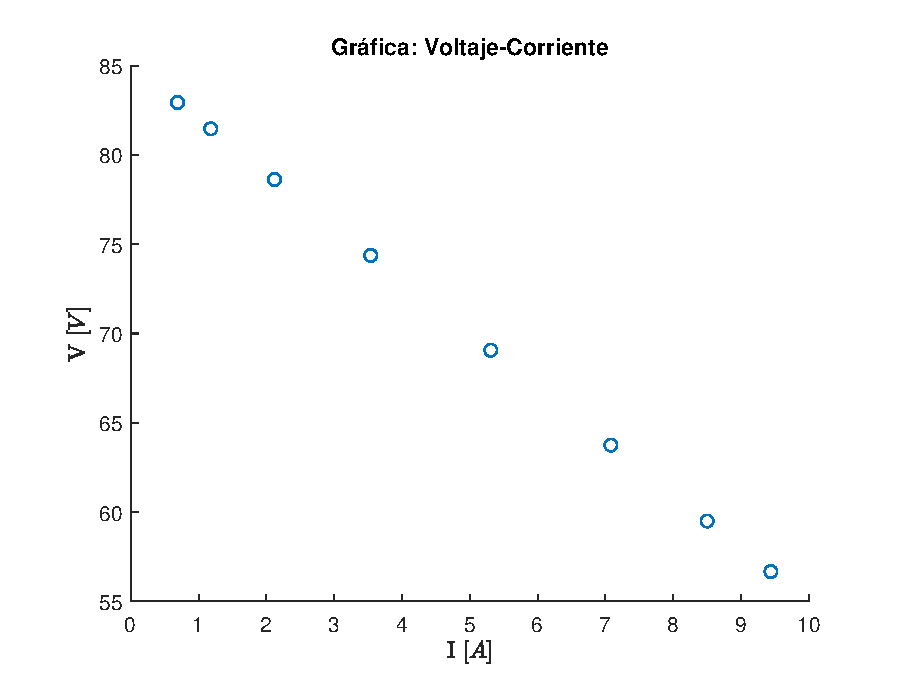
\includegraphics[scale=0.91]{resources/p3.eps}
\caption{Lineas de campo eléctrico para la configuración 3.}
\label{figura10}
\end{figure}

\section{Cuestionario}

\begin{enumerate}
\item \textbf{Comparar las representaciones gráficas obtenidas (líneas
equipotenciales) de las configuraciones utilizadas, con los modelos
teóricos.} \\
Los campos encontrados son similares a los modelos teóricos de campo eléctrico,
existe mayor diferencia con la linea de cargas, al haber utilizado cargas
puntuales con cierta separación, en lugar de electrodos planos.

Siendo ese el caso en el que los campos eléctricos son plenamente paralelas
similar al presentado en la \textbf{Figura \ref{figura11}}.

\begin{figure}[!h]
\centering
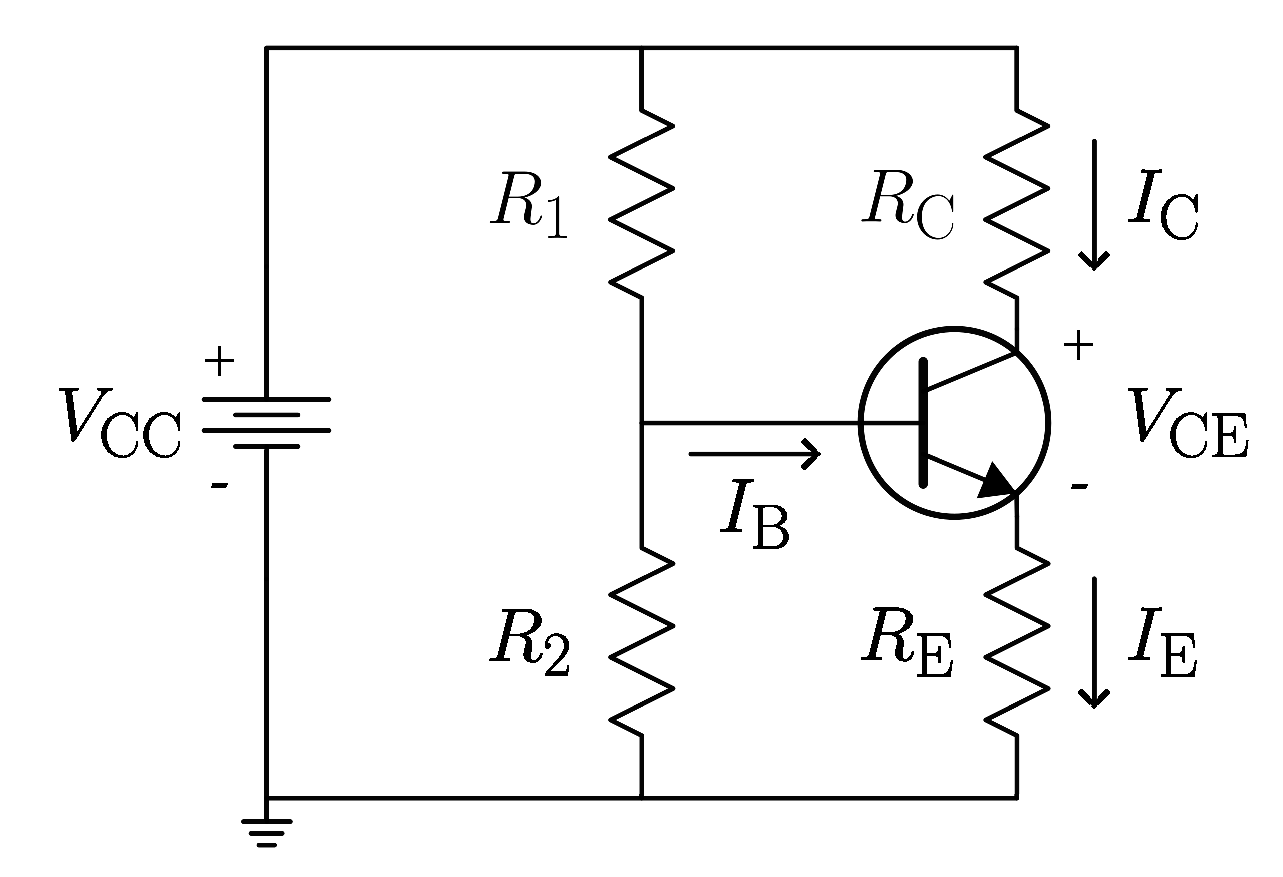
\includegraphics[scale=0.50]{resources/figura11.eps}
\caption{Modelo teórico del campo eléctrico entre dos electrodos planos.}
\label{figura11}
\end{figure}

\item \textbf{A partir del gráfico de las líneas equipotenciales para los
electrodos planos, determinar una relación funcional entre el voltaje $V$ y la
distancia $x$ al electrodo de referencia.} \\

Se tomaron los valores de potencial eléctrico cada $10 [cm]$ en la mitad
de los electrodos planos como se muestra en la \textbf{Figura \ref{figura12}}.

\begin{figure}[!h]
\centering
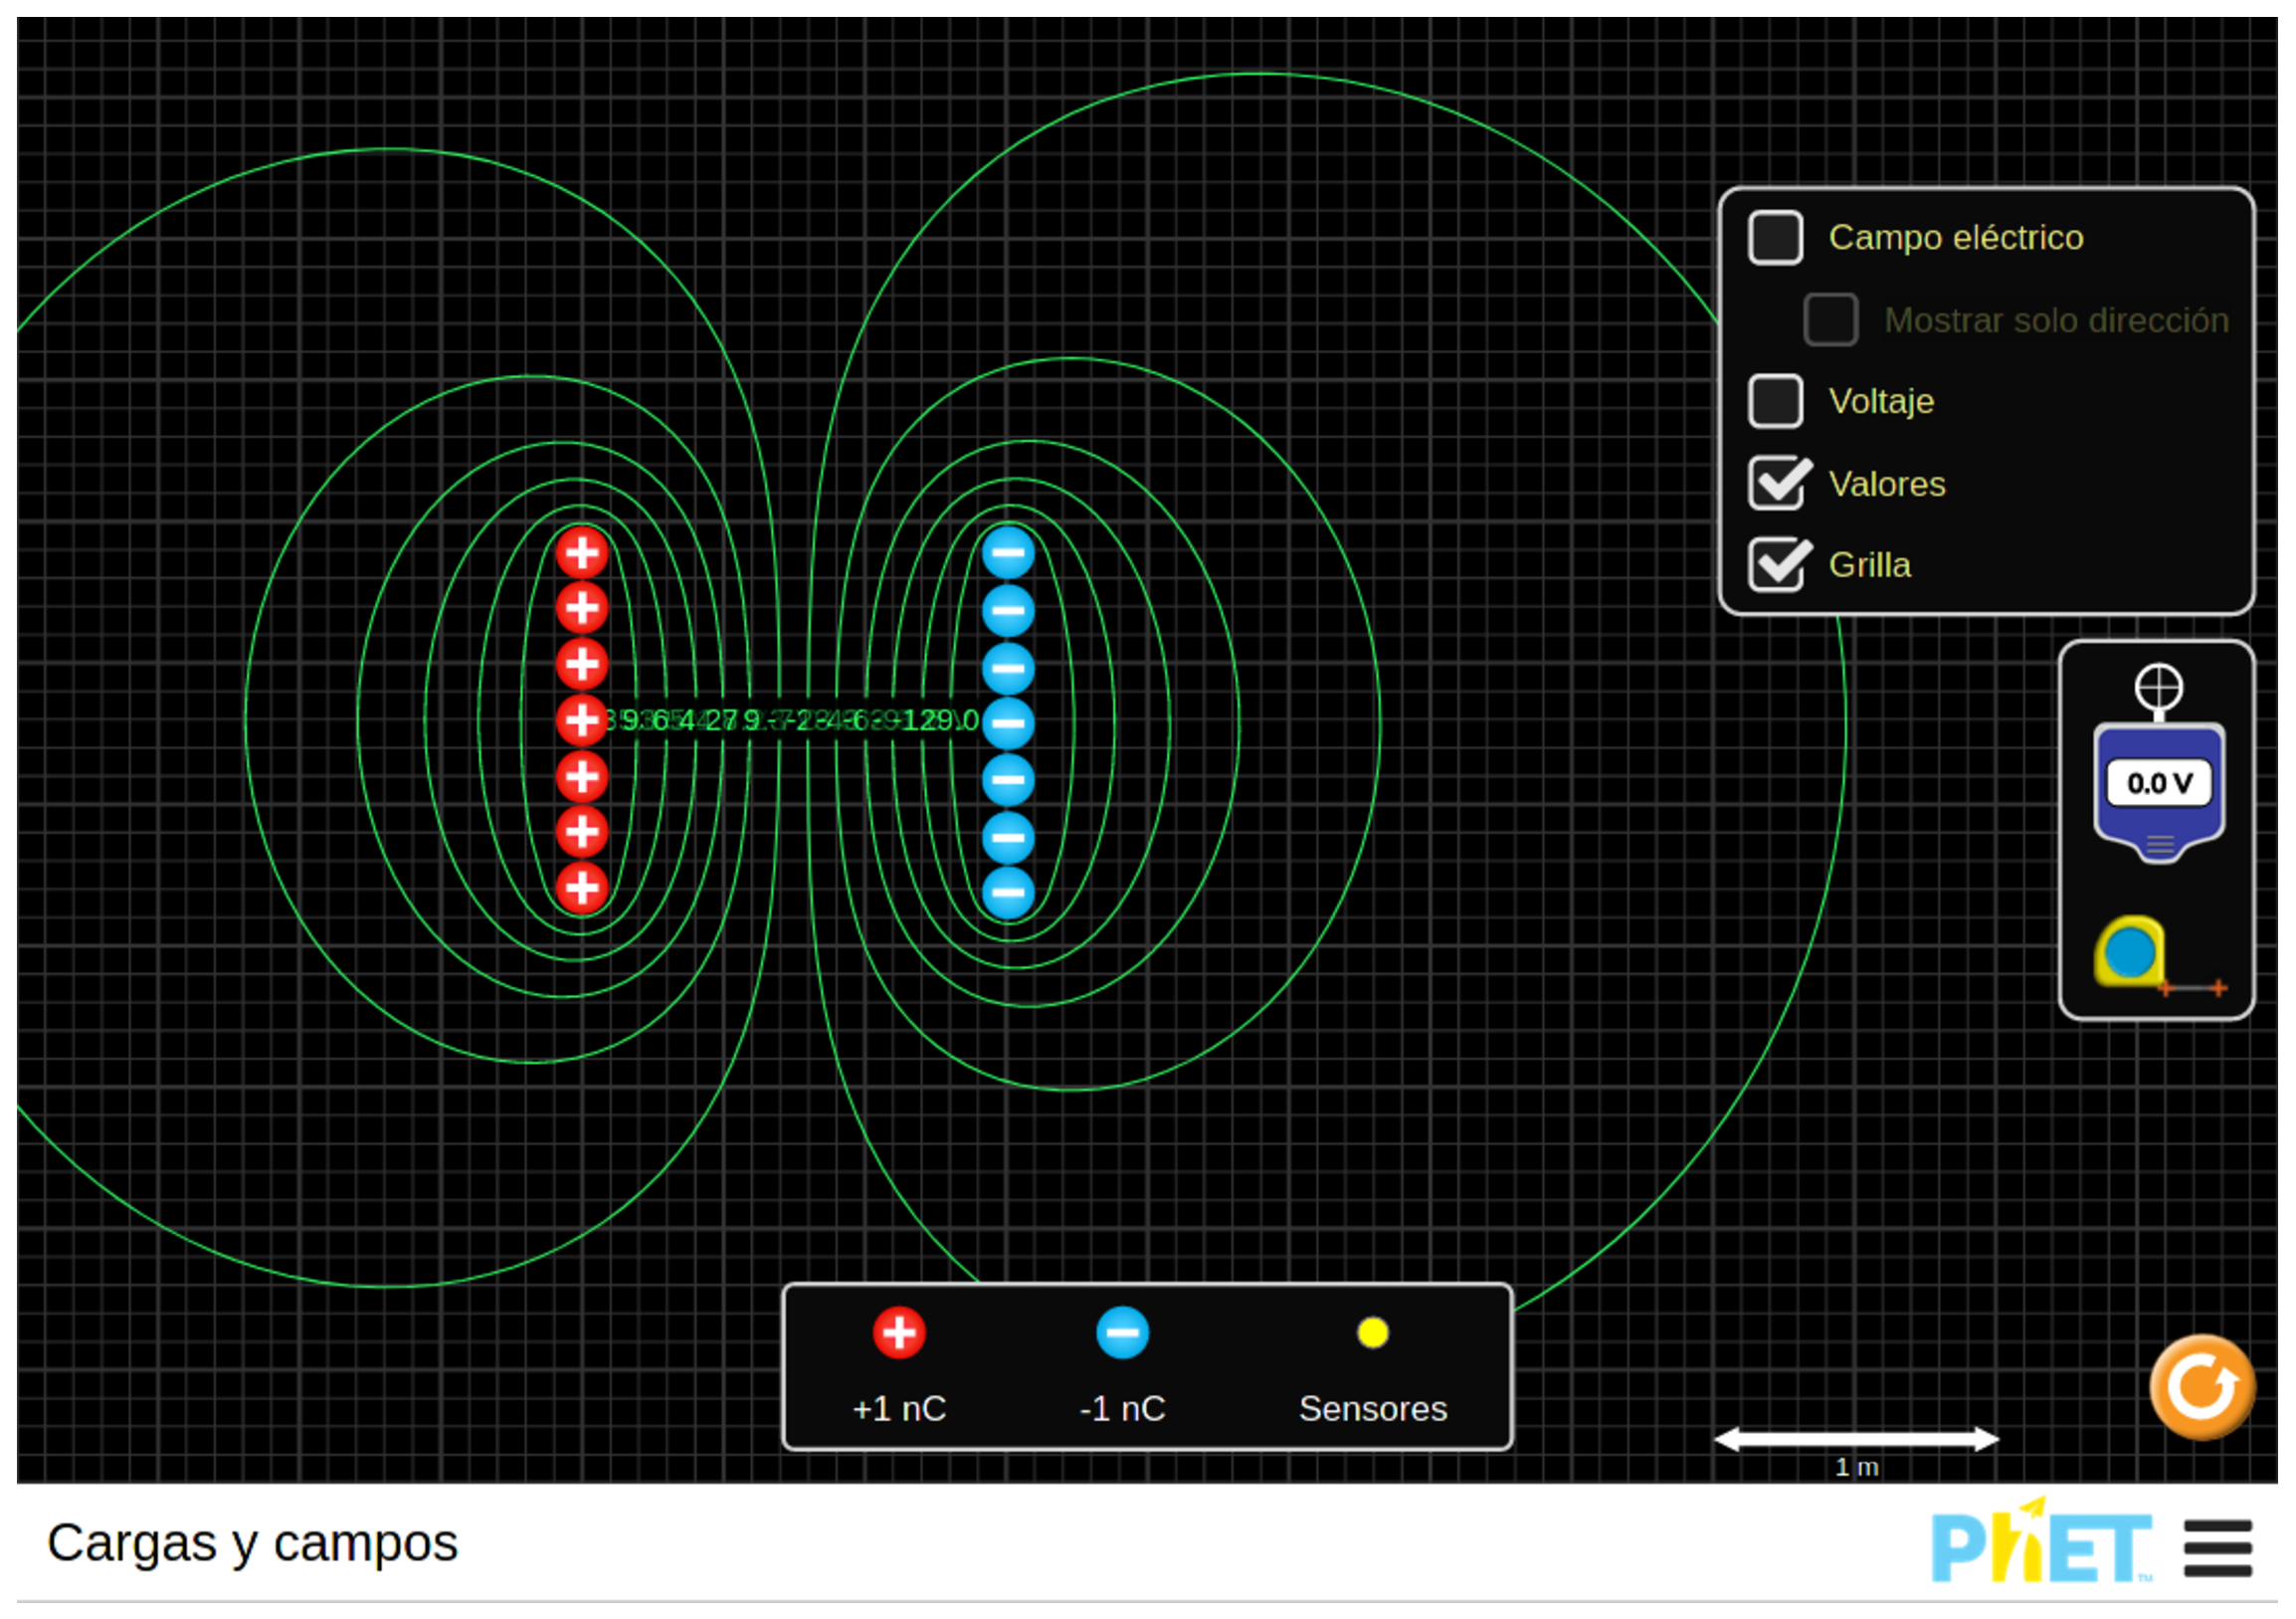
\includegraphics[scale=0.33]{resources/figura12.eps}
\caption{Lineas equipotenciales establecidas en el simulador.}
\label{figura12}
\end{figure}

En el \textbf{Cuadro \ref{cuadro4}}, se presentan los valores de potencial
eléctrico tomados, medidos desde el centro de ambos electrodos planos.

\begin{table}[!h]
\begin{center}
\begin{tabular}{|>{\centering}m{1.0cm}<{\centering}
                |>{\centering}m{1.0cm}<{\centering}
                |>{\centering}m{2.0cm}<{\centering}|}
\hline
$p_i [cm]$ & $n_i [cm]$ & $V_i [V]$ \tabularnewline \hline
 20 & 130 &  135.00 \tabularnewline \hline
 30 & 120 &   93.93 \tabularnewline \hline
 40 & 110 &   65.12 \tabularnewline \hline
 50 & 100 &   44.76 \tabularnewline \hline
 60 &  90 &   27.22 \tabularnewline \hline
 70 &  80 &    9.29 \tabularnewline \hline
 80 &  70 &   -7.03 \tabularnewline \hline
 90 &  60 &  -23.79 \tabularnewline \hline
100 &  50 &  -43.20 \tabularnewline \hline
110 &  40 &  -63.28 \tabularnewline \hline
120 &  30 &  -91.59 \tabularnewline \hline
130 &  20 & -129.00 \tabularnewline \hline
\end{tabular}
\caption{Valores de potencial eléctrico para diferentes distancias.}
\label{cuadro4}
\end{center}
\end{table}

A partir de los datos del \textbf{Cuadro \ref{cuadro4}}, se obtiene la gráfica
presentada en la  \textbf{Figura \ref{figura13}}.

\begin{figure}[!h]
\centering
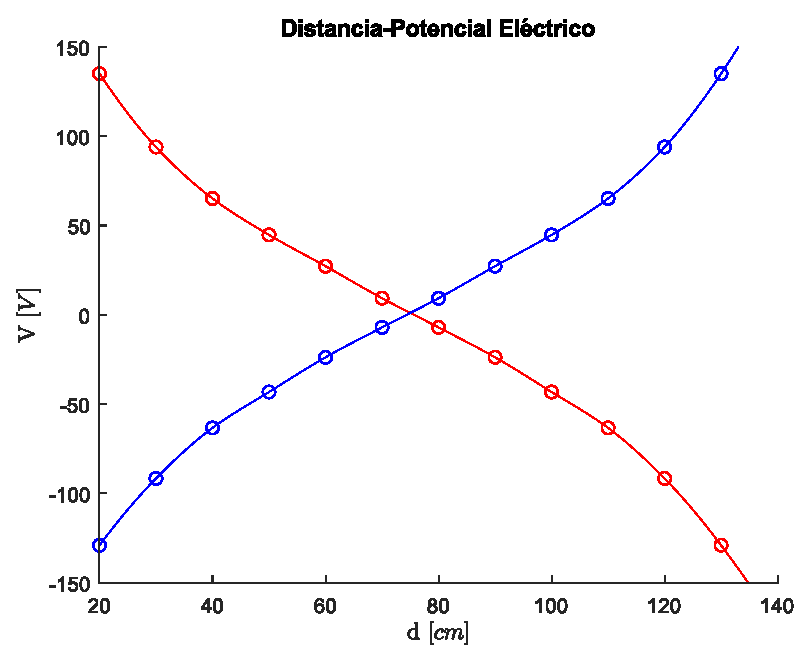
\includegraphics[scale=0.91]{resources/p4.eps}
\caption{Lineas equipotenciales establecidas en el simulador.}
\label{figura13}
\end{figure}

Realizando el ajuste de la curva por el método de los mínimos cuadrados,
obtenemos los valores de la curva y el coeficiente de correlación:

\begin{equation*}
    a = (3119.2 \pm 1426.6)[u]; 45.74 \%
\end{equation*}
\begin{equation*}
    b = (-0.674 \pm 0.1084)[u]; 16.07 \%
\end{equation*}
\begin{equation*}
    R = -0.8914
\end{equation*}

La ecuación de la curva resultante es:

\begin{equation*}
    V = 3119.2 d^{-0.67} - 200
\end{equation*}

Siendo la relación funcional hallada:

\begin{center}
\begin{tabular}{|>{\centering}m{9.2cm}<{\centering}|}
\hline
\textbf{Resultado} 
\tabularnewline \hline
\\
\Large{$V \propto \frac{1}{d^{0.67}}$} \tabularnewline
\\
\hline
\end{tabular}
\end{center}

%\item \textbf{A partir de la relación $V = V(x)$, demostrar: $\nabla^2 V = 0$
%para todos los puntos comprendidos entre las placas.} \\
%\item \textbf{Demostrar la siguiente expresión: $\nabla^2 V = \rho / \epsilon$
%(ecuación de \emph{Poisson}).} \\
%\item \textbf{Si la corriente es estacionaria, se tiene $\nabla \cdot J = 0$.
%Demostrar que para todos los casos se tiene $\nabla^2 V = 0$, y que las líneas
%equipotenciales cumplen esta ecuación.} \\

\end{enumerate}

\end{document}

